\textbf{Входные параметры:}
 
z --- входная переменная.

\textbf{Возвращаемое значение:}
 
Значение функции в точке.

\textbf{Формула:}
\begin{equation*}
f\left(z \right)=\left\lbrace \begin{aligned} 0.5,& \text{ если } \left|z\right| \leq 1 ; \\ 0,& \text{ иначе}. \end{aligned}\right.
\end{equation*}

 \begin{figure} [h] 
   \center
   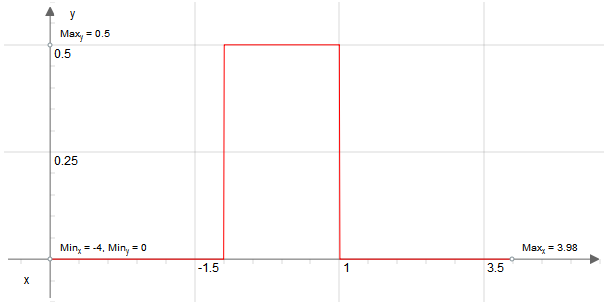
\includegraphics {HML_BellShapedKernelRectangle_Graph.png}
   \caption{График функции} 
   \label{img:HML_BellShapedKernelRectangle_Graph}  
 \end{figure}